\documentclass[pdfCover]{myreport} % 需要pdf封面
% \documentclass{myreport}
\title{测试myreport}
\author{陈伯硕}
\date{\today}

\usepackage{subfiles}
\begin{document}
\maketitle
\pagestyle{empty}
% Generate the Table of Contents if it's needed.
% \tableofcontents
% \newpage

\setcounter{section}{3}
\section{算法设计}
  \subsection{数据结构设计}
    \subsubsection{1}
  \subsection{算法设计}
\section{实验步骤与结果}
  \subsection{代码测试自动机}
    构造自动机类的数据类型和相关方法,
    并检查状态转换是否正确,
    运行
    \begin{lstlisting}[language=python,numbers=none]
    test = Automata('ab')
    test.set_start_state(1)
    test.add_final_states(2)
    test.add_final_states(2)
    test.add_transition(1,2,set(['a','b']))
    test.add_transition(1,3,set('b'))
    test.draw('../docs/figures/test_automata.pdf')
    \end{lstlisting}
    其中打印显示数据类型如下
    \begin{lstlisting}
    {1: {2: {'a', 'b'}, 3: {'b'}}}
    states: {1, 2, 3}
    start state:    1
    final state:    {2}
    transitions:
    1->2 on 'a'
    1->2 on 'b'
    1->3 on 'b'
    \end{lstlisting}

    绘图结果如%
    \cref{fig:automata}
    \begin{figure}[H]
      \centering
      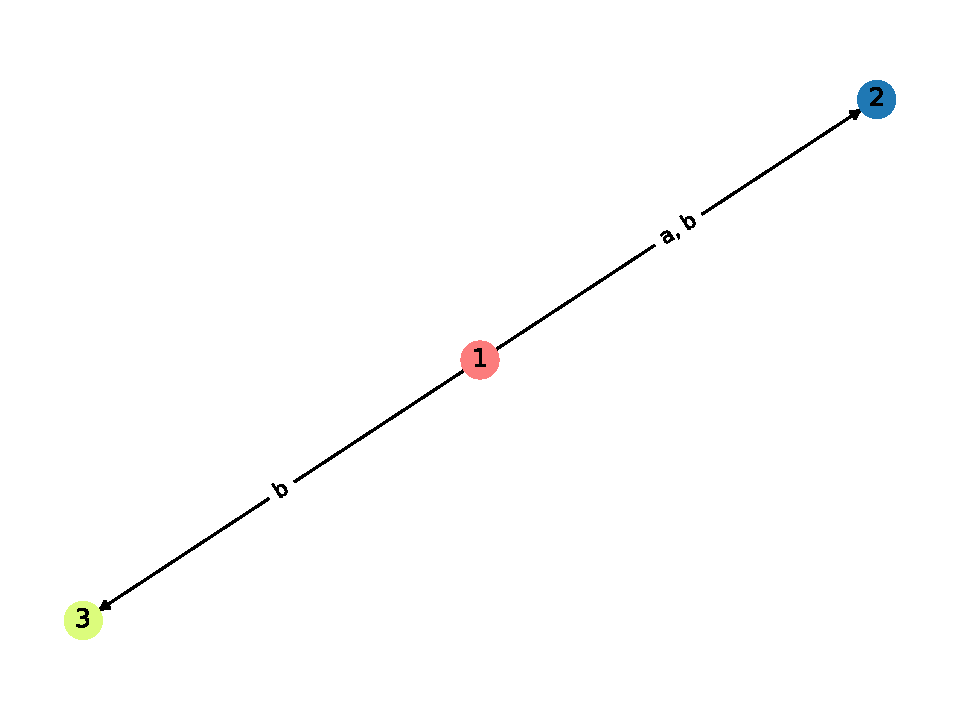
\includegraphics[width = 0.6\textwidth]{test_automata}
      %\missingfigure{automata}
      \caption{测试一个自动机}
      \label{fig:testautomata}
    \end{figure}
    \cref{fig:testautomata}蓝色点代表终态,红色代表初态,其他状态为绿色


\section{实验总结}
% \section{源代码}
% \section{section}
% \subsection{subsection}
% \subsubsection{subsubsection}

% \section{插入代码}
% \begin{codebox}
%   \Procname{$bubble\_sort$($A$: the array, $n$: the length of nums)}
%   \li $a = 1$
%   % \li

% \end{codebox}

\bibliography{reference}
\nocite{alfred_v_aho_compilers_2006}
\nocite{automata-from-regex}

\begin{appendices}
  \section{自动机的相关方法与测试源代码}
    \lstinputlisting[language=python]{../src/Automata.py}
\end{appendices}
\end{document}
